\documentclass[a4paper,12pt]{article}
\usepackage{latexsym}
\usepackage{graphicx}
\usepackage{epsfig}
\usepackage{float}
\usepackage{natbib}
\usepackage{listings}
\usepackage{gensymb}
\graphicspath{{./}}
\DeclareGraphicsExtensions{.png}
\author{Howard Kinsman}
\title{A Multiwavelength Report on Recent Findings on Sgr A*}
\begin{document}
\maketitle
\subsection{Introduction}
Einstein's General Theory of Relativity (GR) predicts the existence of blackholes and the closest and best known candidate is Sgr A* at the centre of the Milky Way. It is believed to be a supermassive 
blackhole (SMBH) and lies at a distance of approximately 8 kpc with an estimated mass of $4\times10^6 M_{\odot}$. It's proximity therefore makes it ideal for the study of blackholes and as a 
potential testbed for GR, as discussed later.
It was first identified as a radio source \citep{balick} back in 1974. It has been studied using the entire electromagnetic spectrum although interstellar extinction makes some wavelengths more 
problematic than others.
Even though, by definition, black-holes are black, they do emit electromagnetic radiation from near the event horizon - as gas and plasma are accreted by the blackhole this material is heated up
and large amounts of energy are emitted and radiated at all wavelengths of the electromagnetic spectrum. However since optical radiation is completely absorbed the best observing bands are radio 
(including sub-mm), the NIR (including far infrared) and X-rays.
The scale of a blackhole is set by the size of the Schwarzschild radius $R_s=2GM_{BH}/c^2\approx 3km (M_{bh}/M_{\odot})$. For Sgr A* this would lead to $\theta_{RS}=10\nu as$  however
for Sgr A* the angular size, affected by gravitational lensing of its own potential, is predicted to be $\approx 10 \mu as$ making it the largest subtended angle blackhole anywhere in the universe and so
is ideal for study. The distance to the Galactic Centre has been determined through high-resolution spectroscopy and the proper motion of stars giving a distance of $D=8.3(\pm 0.4) kpc$.
Apart from mass the other most important parameter of a blackhole is its accretion rate. This is determined by the distance from which it can accrete, the Bondi radius, given by
$R_B=2GM/v_w^2$ where v is the speed of surrounding gas. Estimates for Sgr A* indicate $R_b\approx 2.5\times10^5 R_s \approx 0.1pc$ determined by radio polarization measurements.
Sgr A* has extremely low levels of activity. Its current accretion rate is about four orders of magnitude lower than that required to for a SBMH to grow in a Hubble time \citep{falke1}, its radio emission 
is lower than expected and the amount of gas available as fuel is much lower that required to fuel an SMBH of that size. This has greatly constrained the models of Sgr A*.

This report is a short discussion on recent (2016) findings that have been published on Arxiv with an emphasis on multiwavelength comparisions and the potential for future studies. However the report
begins with a brief summary of the orbits of stars around Sgr A* surveyed over a number of years using the near infrared (NIR) as this data provides some of the most compelling evidence
that Sgr A* is actually a SMBH.

\subsection{Orbiting Stars and Mass of Sgr A* - IR}
The first evidence for a central dark mass was suggested in 1980 through observations from the mid-infrared and radio recombination line observations \citep{falke1}. Although it wasn't until the 
invention of adaptive optics for ground based telescopes that the resolution became sensitive enough to track stars orbiting this mass.
Due to the high levels of exinction when viewing the galactic centre in the optical the NIR has been used to view stars orbiting Sgr A* for decades. There are numerous papers on this subject but this
paragraph begins by citing from \citep{schodel} an early publication on this subject. This survey carried out ten years of high resolution NIR imaging and spectroscopy of the central region of the Milky Way in the
vicinity of Sgr A*. They used an 8m ground-based telescope to study the orbits of S1 and S2, the two closest stars to Sgr A*. S2, the star closest to Sgr A* at the time, was found to be in a
highly elliptical Keplerian orbit with a period of 15.2 years and a peri-centre distance of 17 light hours - at peri-centre S2 was found to have a velocity in excess of 5000 km/s.
From this data they were able to deduce that this orbit would require an enclosed point mass of $3.7\pm1.5\times10^6 M_{\odot}$ at the position of Sgr A*. At this time there were various models
that tried to explain Sgr A* e.g. a dark mass (low mass stars, neutron stars or stellar black holes), a ball of heavy fermions, or a  ball of bosons. This study effectively ruled out the first two of 
these models and put constraints on the possibility of the existence of a ball of bosons. The study was a major first step in testing the SMBH model.
By 2008, 16 years  of stellar orbits of 28 stars had been monitored \citep{gillessen1} using high resolution NIR. This survey combined a long time baseline with high astrometric accuracy using adaptive
optics. This further refined the mass of Sgr A* and showed that a single point mass was the best fit model for this system, pointing again to the SMBH model - see \ref{fig:orbits}

Other evidence that points to the association dark mass wit Sgr A* is its own proper motion. Through VLBI it has been possible to track its motion over several years and its motion has been found to be
entirely consistent with the motion of solar system around the Galactic Centre. This implies the radio source is actually the Galactic Centre.

Today, about 30 stellar orbits have been monitored in the centre of the Milky Way and, combined, this data has yielded the most precise measurement of the mass of Sgr A* as 
$4.23\pm0.14\times10^6 M_{\odot}$ \citep{goddi} with S2 achieving a velocity of 10000 km/s. In 2016 a new methodology of data reduction was piloted \citep{boehle}. They used the star S0-38, which is an
order of magnitude fainter than S2, and so much more difficult to track. The paper illustrates the use of a technique known as speckle holography which allows the speckle imaging data from 1995-2005 to be
re-analysed and fainter stars such as S0-38 to be tracked. The study has put further constraints on both the mass and distance of Sgr A* and reduced the uncertainties to a confidence level of 99.7\%.
The paper hopes that these improved constraints on the gravitational potential in the vicinity of Sgr A*, together with the addition of S0-38, will allow future tests of GR to be carried out when S2
goes through its time of closest approach in 2018. One of the first relatavistic observations for GRAVITY, a second generation instrument on the Very Large Telescope Interferometer (VLTI), an adaptive
optics assisted interferometer, will be to observe the peri-astron shift of S2 in 2018. With a precision of about $10\mu$as GRAVITY will push interferometry accuracy way beyond what is possible today.

\begin{figure}[H]
\centering
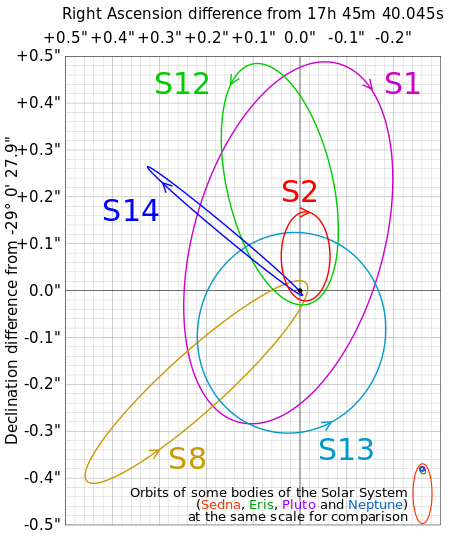
\includegraphics[width=0.75\textwidth]{./orbits}
\caption{Inferred orbits of 6 stars around SMBH candidate SGR A* \citep{eisenhower}}
\label{fig:orbits}
\end{figure}

\subsection{Radio}
As mentioned previously blackholes do emit radiation from around the event horizon due to accretion. It has been calculated \citep{falke2} that the visual appearance of a blackhole would appear as a bright
photon ring with a dim "shadow" within its interior. Photons orbiting very close to the event horizon will disappear into the blackhole whilst those further away will escape to infinity therefore
a clear boundary between light and dark regions is predicted.
Gravitational lensing could increase the size of this shadow to bring it within limits VLBI measurements at mm wavelengths. 
Radio emission from Sgr A* is believed to be produced the accretion onto the SMBH. At millimetre wavelengths, Very Long Baseline Interferometry (VLBI) can resolve the accretion region of the SMBH.
It is believed that this radio emission is either synchotron radiation from a jet outflow, accretion flow onto the SMBH, or an isothermal jet coupled to an accretion flow \citep{ortiz}.
Wavelengths longer than a few centimetres are scattered by the interstellar medium but at smaller wavelengths this scattering is reduced. The scattering obeys a $\lambda^2$ dependence \citep{ortiz} but
at shorter wavelengths this dependence is seen to diminish indicating the structure of Sgr A* may be revealed.
In 2016 a study was carried out to attempt to identify the 2D structure of Sgr A* \citep{ortiz}. Up until this time existing VLBI baselines were limited in the north-south baselines however this study
combined the National Radio Astronomy Observatory Very Long Baseline Array (VLBA) with the Large Millimieter Telescope Alfonso Serrano (LMT) to act a single VLBI array. This provided good north-south as
well as east-west coverage. The study revealed that the image of Sgr A* resembles an elliptical Gaussian. 
A similar VLBI survery was carried out \citep{brinkerink} also using the VLBA, LMT and the Robert C. Byrd Green Bank Telescope (GBT) but this time at a 3mm wavelength using closure phase
interferometry. Closure amplitudes are formed by combining complex ampltitudes in the correlated data from four different telescopes so that the telescope-based gain errors cancel \citep{falke1}.
 They also managed to account for some structure in the Sgr A8 image. The paper describes an Eastern secondary source separate from the primary source, although the authors do
note that this asymmetry may potentially be due to interstellar scattering rather than being intrinisic to the source.
The Atacama Large Millimetre Array (ALMA) is the most sensitive (sub)mm-wave telescope ever builts and consists of 50 individual antennas of 12m diameter. Joint VLBI observations which include ALMA are planned
for 2017 and should provide unprecedented sensitivity due to the improved north-south baseline. Given the overwhelming evidence that Sgr A* lies in the close vicinity to a SMBH there are a number of ongoing observations which aim to test for the existence of blackholes, test GR and study 
spacetime around blackholes \citep{goddi}. Also submm telescopes are combining around the world, icluding ALMA, to form the Event Horizon Telescope (EHT) which should provide unprecedented
sensitivity for VLBI.

The radio spectrum for Sgr A* exhibits a slow rise with frequency until it reaches the submm band where it peaks and then cuts off - this has been termed the "submm bump". It is generally thought that
this is due to synchtron emission in transition from being optically thick to optically thin \citep{falke1}.

\subsection{G2 and Gamma}
A notable, and widely publicised, event occurred in the vicinity of Sgr A* during 2013-14. It was reported \citep{gillessen2} that a gas cloud, now known as G2, of the order three Earth masses, was on
a highly eccentric orbit towards the SMBH and it's predicted pericentre passage would occur late 2013 and would last up to a year. This was again observed using IR. 
This sparked interest in the scientific community as it was assumed that in-falling matter into the SMBH could accelerate
high-energy particles resulting emission at various wavelengths, including gamma rays. A four year observational campaign was therefore started by using the Major Atmospheric Gamma Imaging Cherenkov
(MAGIC) telescopes \citep{ahnen}. These two 17m diameter telescopes record flashes of Cherenkov light produced the Extensive Air Showers which occurr in the upper atmosphere and are caused by very
high energy $\gamma$ ray photons with energies $>50GeV$. The results however were disappointing and the close proximity of G2 to the SMBH had no measureable effect on $\gamma$ ray emissions, although
the authors hope this study will act as a baseline for monitoring any flaring activity in the future. These results, however, are not surpising as it had already been reported \cite{ghez} that G2
had passed by Sgr A* largely unaffected when monitored using NIR.

\subsection{X-ray}
Since the launch of Chandra in 1999 it was found that Sqr A* is a source of suprisingly weak X-rays \citep{falke1}.

\subsection{Multiwavelength}
The flaring activity associated with Sgr A* are also widely studied and observed phenomena. These can be observed using infrared, X-ray and submillimetre wavelengths. The origin of these flares is still
being debated but to understand this activity it is important to compare results from all of these wavelengths. A multiwavelength campaign \citep{mossoux} was therefore carried out in 2014, also timed
to be carried out at G2's closest approach.
This ambitious study aimed to make simultaneous observations using X-Ray Multi-Mirror Mission (XMM-Newton) and Wide Field Camera 3 (WFC3) onboard the Hubble Space Telescope (HST) giving observations in X-Ray and
NIR respectively. NIR observations were also carried out using the Spectrograph for Integral Field Observations in the Near Infrared (SINFONI) at the VLT in Chile. 
Radio observations were also carried using the Karl G. Jansky Very Large Array (VLA) in the X band (3.75-2.5cm) 
and also using the Combined Array for Research in Millimeter-wave Astronomy (CARMA) at 3.2mm. There was no increased flaring activity detected that could be attributed to the passage of G2 however a number of flares
were detected at the various wavelengths allowing the data to be analysed and compared using a multiwavelength approach. 
In total three flares were detected by the WCF3 on board HST plus two more using SINFONIA on the VLT. These were very luminous NIR flares but given that SINFONIA and WFC3 have very high detection limits this
is to be expected statistically. Two X-ray flares were detected by XMM-Newton and were two of the brightest flares ever detected by XMM-Newton. Two of the NIR flares had definite X-ray counterparts
and the one had the highest NIR-to-X-ray ratio ever observed. It seems that X-ray flares are often accompanied by NIR flares but not necessarily vice versa. Data from CARMA revealed a slight 
'bump' but this could not be correlated with any of the NIR/X-ray flares. 
The three main explainations for these flares are: a jet with clumps of ejected material, short-lived "hot spots" orbiting the blackhole or statistical fluctuations in the accretion flow \citep{goddi}.
With its $10\mu$as precision GRAVITY may also soon be able to determine the nature of these flares and settle this debate. GRAVITY should also have the precision to detect Lense-Thirring precession
for stars orbiting the SMBH and hopefully constrain the blackhole spin from stellar orbits.

In a separate study \citep{stone} the Herschel Space Observatory's (no longer operational) Spectral and Photometric Imaging Receiver (SPIRE) was used to carry out the longest ever continuous submillimetre 
survey of Sgr A*. These were observed in three FIR bands: 0.25, 0.35 and 0.5mm. These wavelength are difficult, if not impossible, to observe from the ground. The aim of the study
was to test for the variability of luminosity of the accretion flow into SMBH.
This was then compared with ground-based observations at the Caltech Submillimetre Observatory using 0.85mm and X-ray data from XMM-Newton. Small (<1\%) variations were seen at the three wavelengths
used by SPIRE and comparison with 0.5mm ground data support these small variations. However comparison XMM-Newton didn't reveal any corresponding variations. 

\subsection{Pulsars}
Given the overwhelming evidence that Sgr A* lies in the close vicinity to a SMBH there are a number of ongoing observations which aim to test for the existence of blackholes, test GR and study 
spacetime around blackholes \citep{goddi}. Some very precise tests of GR have been carried out using pulsars: a pulsar in a binary can be used to probe the spacetime around that system by comparing the 
"pulsar clock" with the radio telescope maser. However it is believed that a pulsar orbiting a blackhole could provide an even more accurate test. No such system has yet been found however it is 
believed that there are many pulsars orbiting Sgr A*. The huge mass of SMBH would provide a very accurate test of GR. Unfortunately only five pulsars within 0.5\degree of Sgr A* have so far been found,
the lack of which
has been attributed to interstellar scattering. However in 2013 radio emission from a magnetar (PSR J1745-2900) was detected supporting the hypothesis that many more pulsars may yet still be found. It is
hoped that ALMA will help achieve this aim.
Through the use of modelling \citep{rajwade} state that it is not surpising current surveys have failed to find many pulsars in the Galactic Centre has they have only probed $<2\%$ of the population.
The authors state that upcoming telescopes such as the Square Kilometre Array would probe deepper and survey a more sizeable population of the pulsars in the Galactic Centre.

\subsection{Summary}
This report has so far mentioned three ongoing projects to test GR: the blackhole shadow using EHT, stars orbiting Sgr A* using GRAVITY and pulsars with ALMA. Each of these techniques uses utilises
different wavelengths and observational techniques: mm-VLBI, astrometry with NIR and pulsar timing with radio. It is hoped the combination of these results will test the validity of GR with
more accuracy than ever before. The increasing precision of VLBI observations has prompted some authors \citep{haggard} to suggest that we are approaching the observational limit to where quantum 
gravitational effects may be observed. Sgr A* provides us with the most direct evidence of the existence of blackholes and is by far the closest so ongoing observations at all possible wavelengths are
essential to provide us with more information on the physics of blackholes and ultimately a test of GR in the strong field limit.

\begin{thebibliography}{1}
\bibitem[Balick et al.(1974)]{balick}Balick, B., Brown R. L., (1974), ApJ, 194, 265
\bibitem[Schodel et al.(2002)]{schodel}Schodel, R., Ott, T., Genzel, R., Hofmann, R., Lehnert, M., Eckart, A., et al., 2002, Closest Star Seen Orbiting the Supermassive Black Hole at the Centre of the Milky Way, 
arXiv:astro-ph/0210426v1
\bibitem[Goddi et al.(2016)]{goddi}Goddi, C., Falcke, H., Rezzolla, L., Brinkerink, C. et al., BlackHoleCam: fundemental physics of the Galactic center, arXiv:1606.08879c1, WSPC Proceedings, 2016 
\bibitem[Boehle et al.(2016)]{boehle}Boehle, A., Ghez, A., M., Schodel, R., Meyer, L. Yelda, S. et al, 2016, An Improved Distance and Mass Estimate for Sgr A* from a Multistar Orbit Analysis, 
arXiv:1607.05726v1
\bibitem[Gillessen et al.(2009)]{gillessen1}Gillessen, S., Eisenhauer, F., Trippe S., et al., 2008, Monitoring Stellar Orbits Around the Massive Black Hole in the Galactic Center, The Astrophysical Journal,
692 (2): 1075-1109, arXiv:0910.3069v1
\bibitem[Ortiz-Leon et al.(2016)]{ortiz}Ortiz-Leon, G., N., Johnson, M., D., Doelman, S.,S., Blackburn, L., et al., 2016, The Intrinsic Shape of Sagittarius A* at 3.5mm Wavelength, arXiv:1601.06571v2
\bibitem[Falke, Markoff(2013)]{falke1}Falke, H., Markoff, S. B., 2013, Towards the event horizon - the supermassive black hole in the Galactic Center, arXiv:1311.184v1
\bibitem[Brinkerink et al.(2016)]{brinkerink}Brinkerink, C., D., Muller, C., Falcke, H., Bower, G., C., et al., 2016, Asymmetric structure in Sgr A* at 3mm from closure phase measurements with VLBA, GBT and LMT,
MNRAS, arXiv:1608.0651v1
\bibitem[Gillessen et al.(2012)]{gillessen2}Gillessen, S., Genzel, R., Fritz, T., et al., 2012, Nature, 481, 51
\bibitem[Ahnen et al.(2016)]{ahnen}Ahnen, M.,L., Ansoldi, S., Antonelli, L., A., Antoranz, P., Arcaro, C., et al., 2016, Observations of Sagittarius A* during the pericenter passage of the G2 object with MAGIC, A\&A, arXiv:1611.07095v1
\bibitem[Ghez et al.(2014)]{ghez}Ghez, A., M., Witzel, G., Sitarski, B., et al, 2014, The Astronomer's Telegram, 6110, 1
\bibitem[Mossoux et al.(2016)]{mossoux}Mossoux, E., Grosso, N., Bushouse, H., Eckart, A., Yusef-Zadeh, F., et al., Multiwavelngth study of the flaring activity of Sgr A* in 2014 February-April, 2016,
A\&A, ArXiv:1603.01048v1
\bibitem[Stone et al.(2016)]{stone}Stone, J., M., Marrone, D., P., Dowell, C., D., Schulz, B., et al., Far Infrared Variability of Sagittarius A*: 25.5 Hours of Monitoring with Herschel, 2016, arXiv:1605.05392v1
\bibitem[Haggard, Rovelli(2016)]{haggard}Haggard, H., M., Rovelli, C., Quantum Gravity Effects around Sagittarius A*, 2016, arXiv:1607.00364v2
\bibitem[Falke et al.(2000)]{falke2}Falke, J., Melia, F., Agol, E., 2000, ApJL, 528, L13
\bibitem[Rajwade et al.(2016)]{rajwade}Rajwade, K., M., Lorimer, D., R., Anderson, L., D., 2016, Detecting pulsars in the Galactic Centre, MNRAS, arXiv:1611.06977v1
\bibitem[Eisenhauer et al.(2005)]{eisenhower}Eisnenhower, F., et al, 2005, SINFONI in the Galactic Centre: Young Stars and Infrared Flares in the Central Light-Month, Apj, 628: 246-259
\end{thebibliography}
\end{document} 